%!TEX program = pdflatex
%!BIB program = biber

\listfiles
\documentclass[preprint, nonatbib, 10pt]{elsarticle}

% Fix for using biblatex
\makeatletter
\let\c@author\relax
\makeatother

%-----<<<<<<<<<<<< BIBLIOGRAPHY with biblatex >>>>>>>>>>>>----- 	
\usepackage[backend=biber, style=apa]{biblatex}
\DeclareSourcemap{
  \maps[datatype=bibtex]{
    \map{ % set fields in .bib file to ignore
      \step[fieldset=issn, null]
      \step[fieldset=isbn, null]
      \step[fieldset=abstract, null]
      \step[fieldset=doi, null]
      \step[fieldset=url, null]
    }
  }
}
%
\addbibresource{literature.bib}	% bib file
%-----<<< --------------------------------- >>>-----

%% Packages
\usepackage{lineno,hyperref}
\usepackage[nolist]{acronym}
% \usepackage{natbib}
\usepackage{booktabs}
\usepackage{setspace}
\usepackage{epstopdf}
\usepackage{longtable}
\usepackage{multirow}

%
%
%% Acronyms
\acrodef{BIC}{Bayesian Information Criterion}
\acrodef{BMA}{Bayesian Model Averaging}
\acrodef{BRIC}{Bayesian Risk Inflation Criterion}
\acrodef{CBF}{Conditional Bayes Factor}
\acrodefplural{CBF}[CBFs]{Conditional Bayes Factors}
\acrodef{CSWD}{Credit Suisse Wealth Databook}
\acrodef{DINA}{Distributional National Accounts}
\acrodef{EFW}{Economic Freedom of the World}
\acrodef{FDI}{Foreign Direct Investment}
\acrodefplural{FDI}[FDIs]{Foreign Direct Investments}
\acrodef{GDP}{Gross Domestic Product}
\acrodef{GFDD}{Global Financial Development Database}
\acrodef{HBS}{Household Balance Sheet}
\acrodef{IID}{Independent Identically Distributed}
\acrodef{IVBMA}{Instrumental Variable Bayesian Model Averaging}
\acrodef{LIS}{Luxembourg Income Study}
\acrodef{MCMC}{Markov-chain Monte Carlo}
\acrodef{ML}{Marginal Likelihood}
\acrodef{OECD}{Organisation for Co-operation and Development}
\acrodef{OLS}{Ordinary Least Squares}
\acrodef{PIP}{Posterior Inclusion Probability}
\acrodefplural{PIP}[PIPs]{Posterior Inclusion Probabilities}
\acrodef{PMP}{Posterior Model Probability}
\acrodefplural{PMP}[PMPs]{Posterior Model Probabilities}
\acrodef{PWT}{Penn World Table}
\acrodef{SWIID}{Standardized World Income Inequality Database}
\acrodef{UIP}{Unit Information Prior}
\acrodef{UK}{United Kingdom}
\acrodef{US}{United States}
\acrodef{WALS}{Weighted-average Least Squares}
\acrodef{WB}{World Bank}
\acrodef{WID}{World Inequality Database}
\acrodef{WIID}{World Income Inequality Database}
%
%
\modulolinenumbers[5]

\journal{European Journal of Political Economy}

%%%%%%%%%%%%%%%%%%%%%%%
%% Elsevier bibliography styles
%%%%%%%%%%%%%%%%%%%%%%%
%% To change the style, put a % in front of the second line of the current style and
%% remove the % from the second line of the style you would like to use.
%%%%%%%%%%%%%%%%%%%%%%%

% Numbered
% \bibliographystyle{model1-num-names}

%% Numbered without titles
% \bibliographystyle{model1a-num-names}

%% Harvard
% \bibliographystyle{model2-names}\biboptions{authoryear}

%% Vancouver numbered
% \usepackage{numcompress}\bibliographystyle{model3-num-names}

%% Vancouver name/year
% \usepackage{numcompress}\bibliographystyle{model4-names}\biboptions{authoryear}

%% APA style
% \bibliographystyle{model5-names}\biboptions{authoryear}

%% AMA style
% \usepackage{numcompress}\bibliographystyle{model6-num-names}

%% `Elsevier LaTeX' style, distributed in TeX Live 2019
%\bibliographystyle{elsarticle-num}
% \usepackage{numcompress}\bibliographystyle{elsarticle-num-names}
% \bibliographystyle{elsarticle-harv}\biboptions{authoryear}
%%%%%%%%%%%%%%%%%%%%%%%

\begin{document}

\begin{frontmatter}

\title{Finance and Inequality - panel BMA approach\tnoteref{mytitlenote}}
\tnotetext[mytitlenote]{The author acknowledges support from Charles University Research Centre program No. UNCE/HUM/035.}

%% Group authors per affiliation:
\author[1]{Jan Mare\v{s}}
\ead{janxmares@gmail.com}
\address[1]{IES, Faculty of Social Sciences, Charles University, Opletalova 26, Prague}

%% or include affiliations in footnotes:
% \author[mysecondaryaddress]{Global Customer Service\corref{mycorrespondingauthor}}
% \cortext[mycorrespondingauthor]{Corresponding author}

% \address[mymainaddress]{1600 John F Kennedy Boulevard, Philadelphia}
% \address[mysecondaryaddress]{360 Park Avenue South, New York}

\begin{abstract}
We investigate the impact of financial development on income inequality differentiating between depth, efficiency and access to financial markets and institutions. We apply panel Bayesian model averaging framework to address model uncertainty to reveal that financial development has complex relationship   with the income distribution within countries. The access to and efficiency of banking decrease income inequality. The size of the markets has no relevance for overall income inequality, but relates to the higher top income shares. Moreover, unemployment along with investment into non-tangible assets increase income inequality while more redistribution implies lower levels of inequality.
\end{abstract}

\begin{keyword}
Finance, Inequality, Bayesian Model Averaging
\end{keyword}

\end{frontmatter}

% \linenumbers

\section{Introduction}
\label{ch4sec:intro}
Financial development alters how much the economic opportunities depend on the individual skills, family endowments, social status or political connections as individual may depend on financial system to provide loans to start new business, attain education, or temporarily fund their consumption. The research in the area of financial development and income inequality is well established. \textcite{demirgucc2009finance}, \textcite{claessens2007finance}, and more recently \cite{de2017finance} provide extensive reviews of the topic. A similar theme emerges in all three papers. The implications from theoretical contributions provide conflicting predictions about the relationship and empirical results bring evidence for both positive and negative effect. Although majority of the papers point towards finance tightening the distribution of income this results is not universal with some papers suggesting the opposite while other stress potential non-linearities.

A key divide appears between the effect of financial development on extensive and intensive margin. The extensive margin captures the extend to which individuals, who had not been using financial services before, gain access. On the other hand, the intensive margin describes growing use of finance by the agents who had already been using it before \parencite{demirgucc2009finance}. Financial development on the extensive margin might lead to more equal opportunities and outcomes. Access to credit by previously disadvantaged groups allows human capital accumulation \parencite{galorzeira1993income, galormoav2004, braunetal2019}, formation and growth of new firms \parencite{evans1989estimated,banerjeenewman1990}, with more evenly distributed economic opportunities as a result\footnote{Having similar economic opportunities might decrease the cross-generational inequality, by diminishing the effect of e.g. parental wealth. Depending on the innate abilities and talents of the individuals, however, it may increase the inequality of income within every generation at the same time.}.

On the contrary, intensive margin of financial development might disproportionately benefit the rich who may leverage financial services for their further benefit or to protect their existing rents. \textcite{GreenwoodJovanovic1990} present a model where the finance is the key driver of inequality and the welfare gains accrued by the incumbents - primarily the rich - in the initial development stage. With time, more agents meet the fixed costs of joining the financial intermediaries and they enjoy higher returns. Consequently, the efficiency of resource allocation also increases, which enhances growth and reduces inequality. \textcite{perotti2007investor} present a framework based on political economy. They argument depends on a lobby for lower investor protection to prevent entrance of the new competitors. The politicians require higher bribe from the lobbyist the greater is their accountability for policy decisions. Thus, with increasing accountability, investor protection strengthens and spurs market entry and competition. The authors examine their prediction in a cross-section and show that better investor protection correlates with larger entry rates and higher firm density in more financially intensive sectors\footnote{In addition, they show that the most important factor of accountability is not the formal measure of democratic institutions, but newspaper readership which they interpret as broad awareness of policy choices and their outcomes.}. 

Financial development may also have indirect effect on income inequality through economic growth. \textcite{townsendeueda2006} model how finance interacts with production and allocation of credit. If increased use of finance increases the demand for low- relatively to the high-skilled workers, then it may have equalizing consequences for income distribution. Empirical evidence by \textcite{beck2010big} show that bank deregulation and increased competition in loan provision in the \ac{US} primarily benefited the workers with income below the median. Similarly, \textcite{delis2014} provide evidence of bank deregulation and liberalization tightening the income distribution, although this effect is only present in countries with high-quality institutions. They attribute the effect to the changes in labour market conditions and relatively higher wages and working hours of the low-skilled workers following the reforms. 

A set of distinct papers explores the relationship between inequality and growth while stressing financial markets imperfections driving the outcomes. Income inequality and growth may intersect through varying channels. Accumulation of savings, unobservable effort, and investment project size favor the prediction of growth inducing inequality. Negative impact of inequality on human capital accumulation, entrepreneurial activity provide argument for the opposing view. 
\textcite{milanovicvan2018inequality} report how income inequality in the \ac{US} has different implications for the future income growth of the rich and the poor. High inequality seems to hurt the prospects of the poor while the top of the distribution is unaffected. The rich thus disproportionately benefit from higher inequality as their subsequent income exhibit faster growth. The authors attribute this effect to the political channel the rich use to lobby in favor of the policies which support their economic interests. Preferences of the rich are ultimately more likely to determine public policy than the preferences of the majority \parencite{gilens_page_2014}. High inequality together with a credit constraint and rich driving the political process results in low government spending and lasting inequality.

The literature does not converge on the conclusions even in the empirical cross-country and panel data studies. The papers link higher levels of financial development with lower levels of inequality \parencite{beck2007finance, hamori2012, gimet2011closer, kunieda2014finance}\footnote{For an extended list, we refer to \textcite{de2017finance}.}. On the other hand, several other estimate a inequality inducing effect of finance \parencite{Jaumotte2013, jauch2016financial, de2017finance}. Finally, some authors claim there the relationship might be non-linear, conditional on a threshold value of financial development \parencite{kim2011nonlinearity,tan2012nonlinear} or institutional quality \parencite{LawSingh2014, delis2014}.

Three papers are the closest to ours, each in a different respect. First, \textcite{de2017finance} examine different dimensions of finance on income inequality. Their results suggest that financial development, financial liberalization, and banking crises all increase pre-tax income inequality within countries. Additionally, they show that the effect of financial liberalization is conditional on democratic accountability. Higher accountability mitigates the impact of liberalization on inequality. On the contrary, the financial development, proxied by the credit to GDP ratio, has inequality increasing effect irrespective of the institutional background. Second, \textcite{naceurzhang2016} take similar approach in considering multiple dimensions --- the access, efficiency, and stability of the financial sector, although not examining the indicators simultaneously.  Third, \textcite{furceri2019robust} apply \ac{WALS} to identify robust determinants of income inequality. Their approach mirrors ours in accounting for model uncertainty in the estimation. Their focus is more general rather than focused primarily on finance. We provide synthesis and extension to these papers in providing more detailed view on the link between finance in shaping income inequality and examining multiple measures of inequality while specifically identifying the determinants of top income shares along with the determinants of the overall income distribution\footnote{Captured by income Gini index.}.

% An exemption from focus solely on the size of financial sector is the study by \textcite{naceurzhang2016} which applies a similar approach to ours, taking into consideration the access, efficiency, and stability of the financial sector. However, there are severe limitation to their study. First, their coverage does not correspond to the availability of the data. Second, they do not account for the different dimensions of finance simultaneously and always use a single indicator of development at a time. Third, they do not explicitly differentiate between the banking sector and financial markets. We provide a more detailed as well as more robust picture of the financial development effect on finance in these dimensions.

% \textcite{de2017finance} examine different dimensions of finance on income inequality. Their results suggest that financial development, financial liberalization, and banking crises all increase market income inequality within countries. Additionally, they show that the effect of financial liberalization is conditional on democratic accountability. The higher the accountability, the less severe is the negative impact of liberalization on inequality. On the contrary, the financial development, proxied by the credit to GDP ratio, has inequality increasing effect irrespective of the institutional background.

% \textcite{furceri2019robust} apply WALS to identify robust determinants of income inequality. They are the closest paper to ours since they account for model uncertainty in the estimation. Their focus if more general rather than on finance specifically. Out work offers more detailed contribution in terms of the role of finance in shaping income inequality. On the top of that, we differ from their analysis by examining multiple measures of inequality and specifically identifying the determinants of top income shares along with the determinants of the overall income distribution represented by income Gini index. We provide further evidence in all these dimensions.

%
%
%
%
%

\section{Data and methodology}
The key variable in the paper is the measure of income inequality. We want to examine how financial development affects income inequality and whether the effect might by different at the top quantiles of income distribution. As the overall measure of income inequality, we rely the after-tax Gini coefficient from \ac{SWIID} by \textcite{Solt2019}, which is a standard resource in the literature\footnote{There are alternative sources of for Gini coefficient, e.g. \ac{WIID} or \ac{LIS}, but each of them brings limitations in terms of comparability or coverage.}. Its critical advantage lies in the widespread coverage across countries and time and a unified methodology which provides a reasonable level of comparability. It typically takes values in the interval between 0 and 100 where the former suggests perfect equality (everyone in the economy enjoys the same income) and the latter perfect inequality (all the income goes to only a single unit). We depart from existing papers slightly in considering the after-tax rather than the before-tax income distribution as a dependent variable. 

To explore the relationship in the top part of the distribution, we choose top income share from \ac{WID}\footnote{The methodology and guidelines to database are provided by \textcite{alvaredo2016distributional}.}. The surveys suffer from well-known issues of underrepresentation of the top income earners and the distortions resulting from self-reported character of the data. This can influence not only the top income shares resulting from survey data, but also distortions in the overall measures of inequality. The data in \ac{WID} make use of income tax records in individual countries and the derived shares obtained using consistent methodology of \ac{DINA} are arguably more reliable relative to the survey-based measures which are the primary source of majority estimates of income distributions. 

The data spans from 2000 to 2014. We follow the literature \parencite{dabla2015causes,de2017finance} and average both the inequality measure (dependent variable) and the potential determinants (independent variables) across three year intervals. There are important reasons for looking at the averages than observation in individual years. Annual macroeconomic data are subject to fluctuations and the data on income inequality is noisy \textcite{delis2014}. Averaging should diminish the level of noise. On the top of that, the variables at the center of our analysis, e.g. stock market capitalization or credit to \ac{GDP}, are likely to be affected by the business cycles and volatile on the yearly basis. Similar argument holds for top income shares, as they depend, among other things, on the bonuses paid out each year and capital income. We want to explore the long-term rather than the short-term relationship and that guides the choice of averaged data. Faced against the trade-off between length of the averaging periods and available observations in the time dimension, we take a compromise of three years in contrast to the literature, where generally the 5-year intervals apply. The availability of financial development indicators limits the analysis to a period from 2000 onward and we prefer to keep at least 5 unique time periods to just three under the case of 5-year average\footnote{Nevertheless, we run the estimation with 5-year averages of data as a robustness check and find no critical qualitative differences compared to the baseline.}.

Table \ref{ch4tab:sum} report the summary statistics of the income inequality variables and financial development indicators.

% \begin{table}[ht!]
%     \small
%     \caption{Summary statistics of inequality variables}
%     \label{ch4tab:ineq}
%     \centering
%        \begin{tabular}{lrrrr}
%         \toprule
%         Variable & Mean & St. Dev. & Min & Max \\
%         \midrule
%         After-tax Gini index  & & & & \\
%         Top 10\% income share & & & & \\
%         Top 1\% income share & & & & \\
%         \bottomrule
%     \end{tabular}
% \end{table}

\begin{table}[ht!]
  \small
  \caption{Summary statistics of selected variables}
  \label{ch4tab:sum}
  \centering
     \begin{tabular}{lrrrr}
      \toprule
      Variable & Mean & St. Dev. & Min & Max \\
      \midrule
      After-tax Gini index  & 36.38 & 8.12 & 22.88 & 61.16 \\
      Top 10\% income share & 0.42 & 0.12 & 0.24 & 0.71 \\
      Top 1\% income share & 0.14 & 0.06 & 0.05 & 0.38 \\
      FIA & 0.42 & 0.32 & 0.01 & 1.00 \\
      FIE & 0.60 & 0.13 & 0.11 & 0.81 \\
      FID & 0.37 & 0.30 & 0.01 & 1.00 \\      
      FMD & 0.33 & 0.32 & 0.00 & 0.99 \\
      \bottomrule
  \end{tabular}
\end{table}
%
%
%
%
%

\begin{table}[ht!]
  \small
  \caption{Correlation matrix of selected variables}
  \label{ch4tab:corr}
  \centering
  \begin{tabular}{lrrrrrrr}
    \toprule
  %  & GiniNet & Top10share & Top1share & FIA & FIE & FID & FMD \\
    % \midrule
    After-tax Gini index  & . &  &  &  &  &  &  \\
    Top 10\% income share & 0.47 & . &  &  &  &  &  \\ 
    Top 1\% income share & 0.39 & 0.84 & . &  &  &  &  \\
    FIA & -0.14 & -0.09 & -0.12 & . &  &  &  \\
    FIE & -0.14 & -0.10 & -0.06 & 0.28 & . &  &  \\ 
    FID & -0.07 & 0.12 & 0.06 & 0.60 & 0.24 & . &  \\
    FMD & 0.03 & 0.2 & 0.13 & 0.36 & 0.1 & 0.40 & . \\ 
     \bottomrule
  \end{tabular}
  \end{table}

We obtain the financial development indicators from \ac{GFDD}. The database offers detailed indicators along four dimensions of financial systems and allows to estimate the affect of changes in access, size, efficiency, and stability of financial markets. Furthermore, we can distinguish between banking sector and financial markets in all these dimensions. The data in for access and stability of stock markets remains sparse in the concerned period we must leave them out of analysis. We use the version of financial indicators from \cite{svirydzenka2016introducing}. The authors make use of principal component analysis in order to construct aggregate indicators in each characteristic of financial sector. In summary, we have indicators of financial institutions depth (FID), financial markets depth (FMD), access to financial institutions (FIA), efficiency of financial markets (FME), and institutions (FIE)\footnote{\textcite{svirydzenka2016introducing} extrapolate the indicators from top to bottom if the original variables are unavailable, we make sure that that at least one variable is available for the construction of the index and no artificial correlation introduced to the data.}. We report the composition of each indicator in Table \ref{ch4tab:finind}. 

\begin{figure}[ht!]
  \centering
  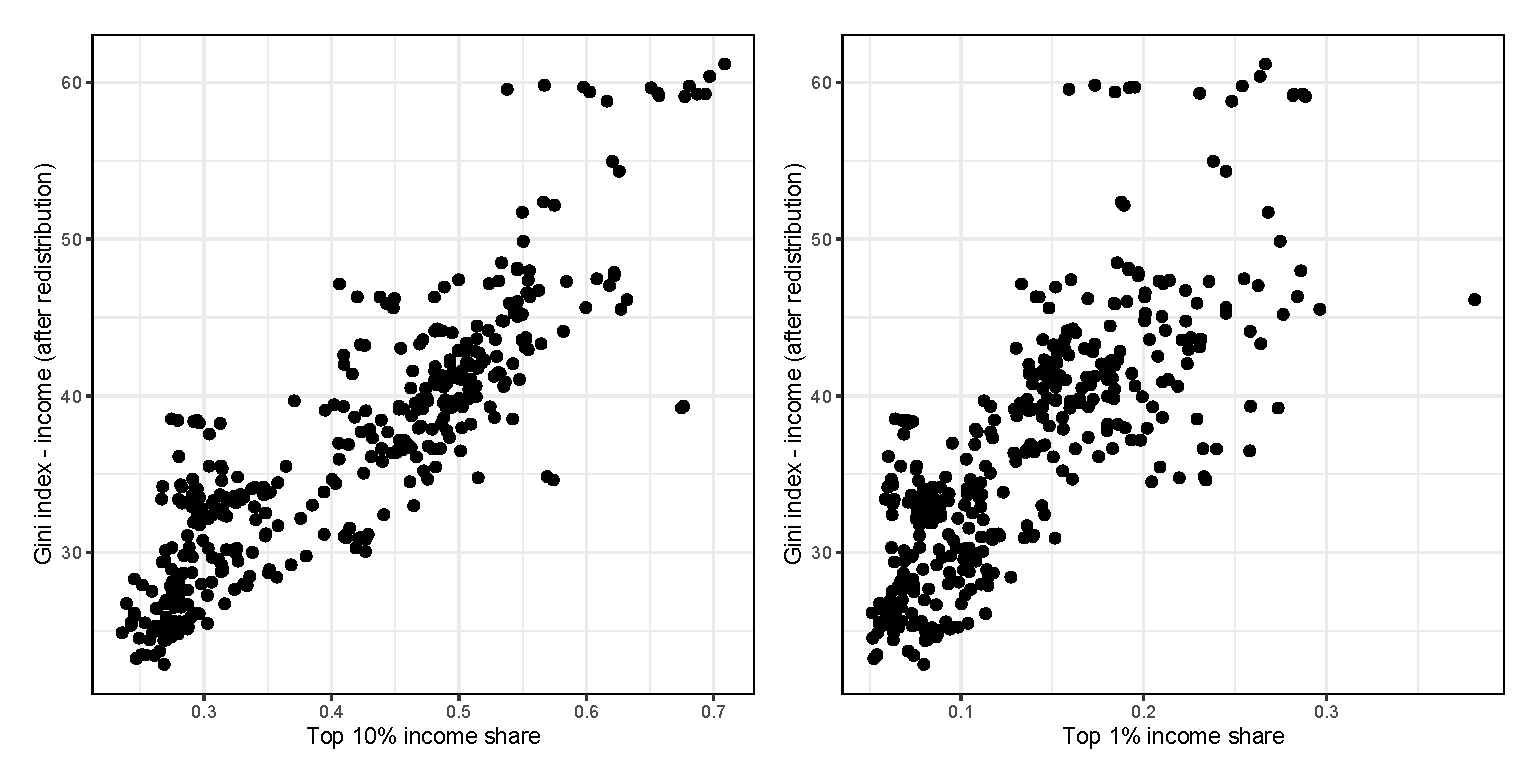
\includegraphics[width=0.8\textwidth, keepaspectratio]{figures/plots_ineq}
  \caption{Gini Coefficient and top shares}
  \label{ch4fig:gini_topshares}
\end{figure}

% Figure \ref{ch4fig:gini_findev} shows the scatter plots of all the available observations after averaging between Gini coefficient and selected financial indicators. Although the data is noisy, it suggest negative correlation between the variables. Figure \ref{ch4fig:gini_findev_dm} then shows the corresponding scatter plots of the data which was demeaned using the within country averages over time. %The relationship between Gini and financial indicators appears considerably weaker following the transformation, with the exception of access to financial institutions where visual inspection allows pointing to a negative correlation.

We build the choice of other explanatory variables on a reviews of income inequality drivers \parencite{roineetal2009,nolan2019drivers}, related study of finance-inequality nexus \parencite{de2017finance}, and a more general inquiry into the robust determinants of income inequality \parencite{furceri2019robust}. The potential regressors could be categorized in several groups. They control for economic and financial development, demographics, globalization, and institutional background. Table \ref{ch4app:exog} reports all the control variables and their sources. 

% \textcite{nolan2019drivers} bring a survey of the literature on determinants of inequality, summarizing the complexity of the inequality dynamics. They stress that many of the determinants are interlinked which implies difficulty in assigning precise effects to individual drivers of inequality. Additionally, they encourage complementary individual country case studies to support the finding of the general cross-country estimates.
% Both theoretical and empirical studies leave out the issue of importing the financial services from abroad. We include financial globalization from KOF among our control variables.
%
%
% \section{Methodology}
% \label{ch4sec:methodology}
Methodologically, we rely on the \ac{BMA} approach which conveniently addresses the issue of model uncertainty with a large number of potential regressors. The advantages are statistical properties of the \ac{BMA} have been sketched in \textcite{Koop2003}. In application to the panel data, we make use of Frisch-Waugh-Lovell theorem and demean all the variables using time averages for individual observations. Using the time-demeaned observations in the estimation is equivalent to the estimate using the dummy variables for individual cross-sectional units. The key assumptions in \ac{BMA} are on parameter and model priors. For the parameter prior, we turn to so-called hyper-g prior. The prior provides more robust results than some other traditionally applied $g$ priors such as \ac{UIP}, \ac{BRIC} \parencite{feldkircher2012impact}. As for the model priors, the baseline estimate relies on the uniform model prior. We choose the model prior to remain agnostic about the prior probability of each examined model. While uniform prior assigns the same prior probability to each model, the distribution of the prior model space is concentrated around $k/2$, where $k$ is the number of potential covariates, and it may consequentially gravitate towards larger model sizes and higher number of covariates\footnote{See \textcite{LeySteel2009} for details.}.

\section{Results}
\label{ch4sec:results}
We examine the determinants of inequality in the panel \ac{BMA} framework and present the results in the following sections. We start with a model where we capture the overall inequality by Gini index in subsection \ref{ch4subsec:gini}. We then continue to estimations where we consider the shares of income going to the top 10\% and top 1\% of the income distribution as our dependent variable. We check the robustness of our estimates by employing alternative model and parameter priors throughout the analysis.

\subsection{Gini index of income distribution}\label{ch4subsec:gini}
We focus the analysis on the relationship between the indicators representing various aspects of financial development and income inequality. Figure \ref{ch4fig:gini_findev_dm} outlines the expected link after we have demeaned the variables using the cross-sectional averages. The relationship is not particularly strong, but we observe negative correlation between Gini index and indicators of access and efficiency of financial institutions, as suggested by a linear estimate. For size indicators of financial market and institutions, the link appears much weaker.

\begin{figure}[ht!]
  \centering
  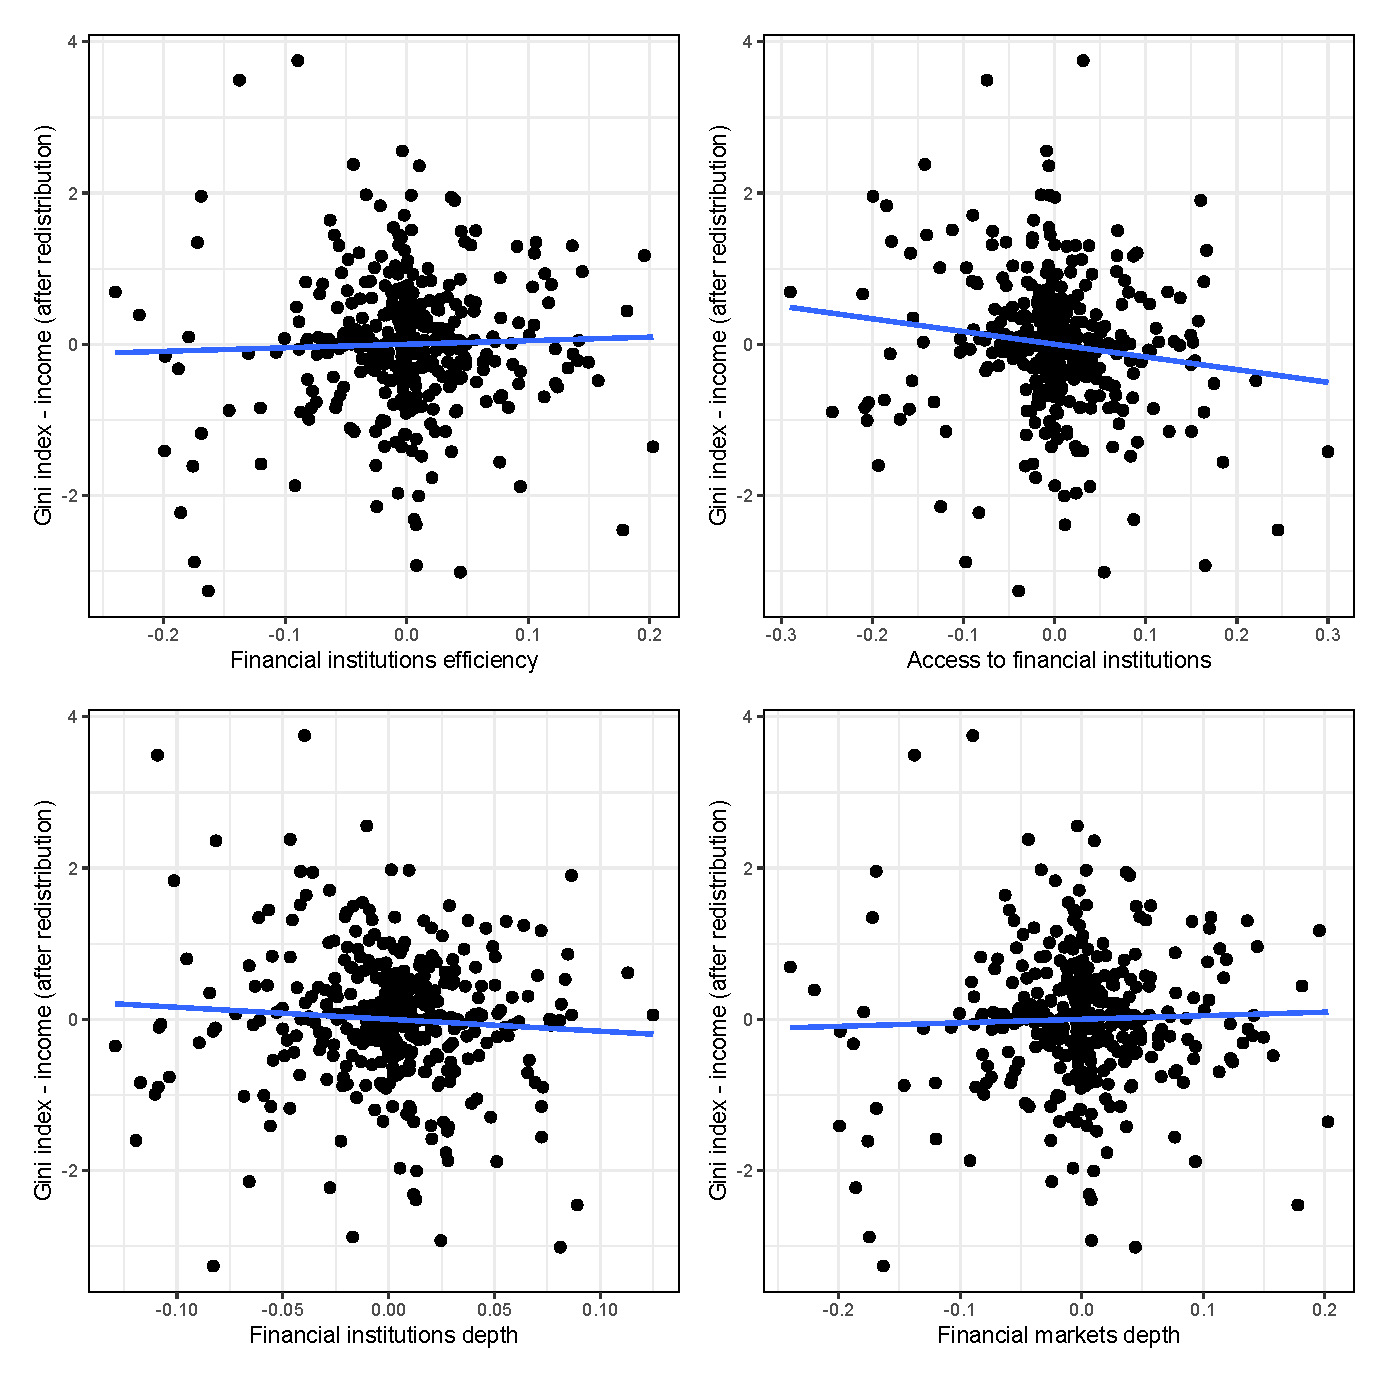
\includegraphics[width=0.8\textwidth, keepaspectratio]{figures/plots_findev_gini_dm}
  \caption{Gini Coefficient and Financial Development Indicators}
  \label{ch4fig:gini_findev_dm}
\end{figure}

% \begin{figure}
%   \caption{Gini Coefficient and Financial Development Indicators}
%   \label{ch4fig:gini_findev}
%   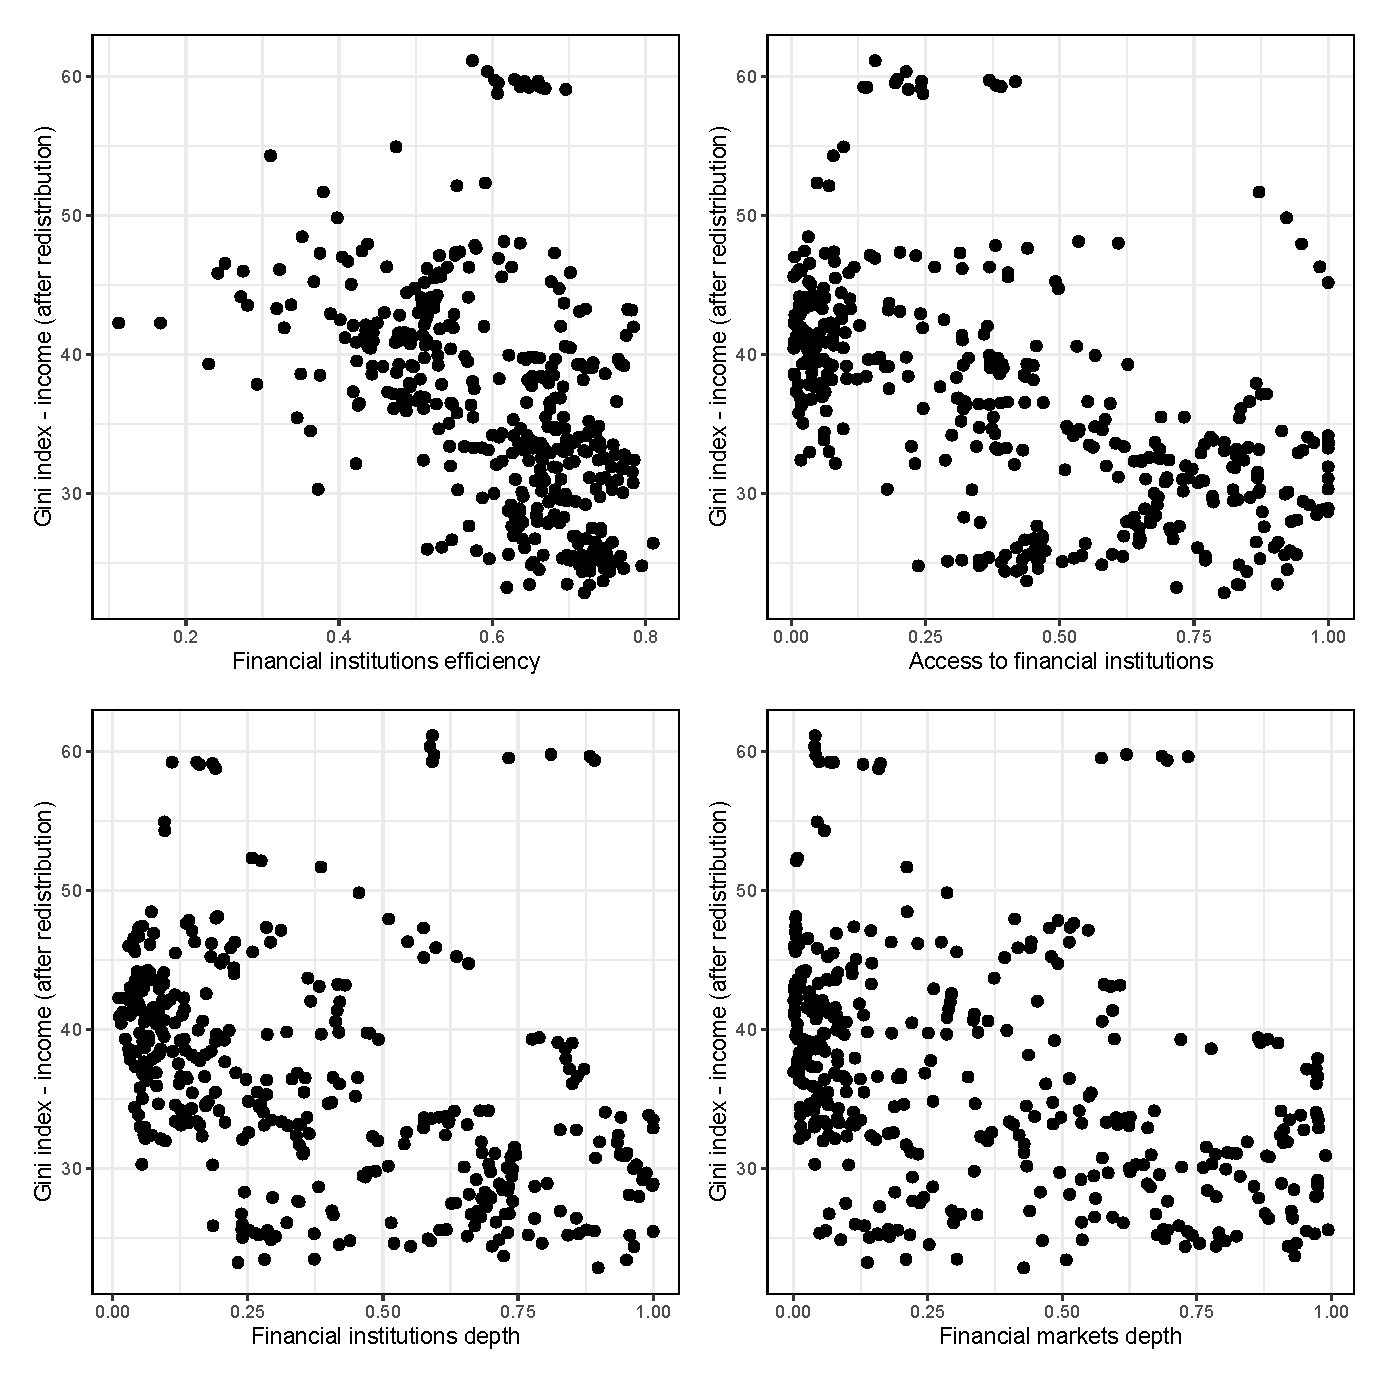
\includegraphics[width=\textwidth, keepaspectratio]{figures/plots_findev_gini}
% \end{figure}

Table \ref{ch4res:baseline_gini} reports the baseline results. Overall, we have 16 variables with \ac{PIP} above 0.8. The number of unique relevant regressors effectively shrinks by two if we abstract from the quadratic terms of the \ac{GDP} per capita and the education index. Most of the estimated posterior means exhibit expected signs.

The only financial indicators which occur among the top regressors are access and efficiency of financial institutions with \acp{PIP} of 1 and 0.88, respectively. The posterior mean on the coefficients in both dimension is negative so higher levels of access and efficiency are associated with lower levels of income inequality. The inequality decreasing effect of access to finance on inequality mirrors \textcite{hasan2020finance} for wealth inequality, and partially also \textcite{furceri2019robust, naceurzhang2016} who document similar effect. The observation on inequality decreasing effect of access to finance supports also \textcite{claessens2007finance} who suggest that access may equalize economic opportunities and lead to more evenly distributed income as well as theoretical predictions \parencite{braunetal2019,galormoav2004,banerjeenewman1990}. The efficiency of financial intermediation putting downward pressure on income inequality also has a precedent in \textcite{gimet2011closer}\footnote{The authors measure efficiency of banking sector by the difference between lending rate and the deposit rate (spread). They argue higher spread reflects low competition and high transaction costs. The imperfections in the credit market can skew the credit to high-income, rich households who can provide significant collateral, reinforcing the existing inequality.}. We fail to confirm that the efficiency of financial institutions is a robust determinant of inequality, however, as the \ac{PIP} markedly decreases under alternative model priors. None of the size indicators of financial institutions or markets has high probability of inclusion.

Education expenditures (\% share of \ac{GDP}) along with the education index calculated using mean and expected years of schooling show inequality decreasing effect. This is in line with prediction of \textcite{goldin2009race,deaton2013great} who claim that the skill-biased technological change should be mitigated by education. \textcite{oecd2011divided} finds similar evidence for a panel of advanced countries while \textcite{furceri2019robust} also suggest a negative relationship, although it is not fully robust to variable and sample selection. The effect of education diminishes at the higher levels of schooling as the quadratic term has also high \ac{PIP} and positive posterior mean. 

\begin{table}[ht!]
  \caption{BMA, baseline results. Dependent variable after-tax Gini index, 394 observations.}\label{ch4res:baseline_gini}
  \footnotesize
  \centering
  \begin{tabular}{lrrr}
    \toprule
                           & PIP & Post Mean & Post SD \\
    \midrule
    Education expenditures & 1.00 & -0.14506 & 0.05042 \\
  GDP per capita & 1.00 & 1.62811 & 0.56870 \\
  Unemployment & 1.00 & 0.23629 & 0.05907 \\
  Non-equipment investment & 1.00 & 0.14977 & 0.05285 \\ 
  Access to financial institutions & 1.00 & -0.24629 & 0.06342 \\
  Education index (UN) & 1.00 & -0.58853 & 0.23865 \\ 
  Redistribution & 1.00 & -0.22055 & 0.05051 \\
  Education index sq. & 1.00 & 0.82252 & 0.22008 \\
  GDP per capita sq. & 1.00 & -1.44906 & 0.57565 \\
  Life expectancy & 0.99 & -0.22879 & 0.09750 \\ 
  Economic freedom & 0.99 & 0.18518 & 0.06941 \\
  Value added in agriculture & 0.97 & -0.12361 & 0.05947 \\
  Government expenditures & 0.95 & 0.12259 & 0.05743 \\ 
  Total population & 0.95 & -0.15378 & 0.08478 \\
  Financial institutions efficiency & 0.88 & -0.08374 & 0.05599 \\
  Inflation & 0.86 & 0.16879 & 0.12487 \\
  \midrule
  Inflation sq. & 0.66 & -0.11127 & 0.11201 \\ 
  Value added in industry & 0.62 & -0.05825 & 0.06407 \\
  Equipment investment & 0.44 & -0.03383 & 0.05359 \\ 
  Financial markets depth & 0.27 & 0.01554 & 0.03673 \\ 
  Gross domestic savings & 0.27 & -0.02022 & 0.04597 \\
  % Period 4 & 0.25 & 0.01282 & 0.03330 \\ 
  Social globalization & 0.23 & 0.02365 & 0.06279 \\
  Restrictions on globalization & 0.15 & 0.00874 & 0.03214 \\
  Trade openness & 0.13 & 0.00615 & 0.02589 \\
  Left-wing orientation & 0.11 & 0.00339 & 0.01720 \\ 
  Rule of law & 0.10 & -0.00333 & 0.01812 \\ 
  Net FDI (\% GDP) & 0.10 & -0.00283 & 0.01575 \\ 
  Natural resources rents & 0.08 & -0.00223 & 0.01583 \\ 
  Chinn-Ito index & 0.07 & -0.00205 & 0.01780 \\ 
  % Period 5 & 0.07 & 0.00025 & 0.02188 \\ 
  % Period 2 & 0.07 & 0.00133 & 0.01321 \\
  % Period 3 & 0.06 & -0.00027 & 0.01423 \\
  Financial globalization & 0.06 & -0.00134 & 0.01466 \\
  Civil liberties \& political rights & 0.06 & 0.00075 & 0.01131 \\ 
  Financial institutions depth & 0.05 & 0.00060 & 0.01316 \\ 
  GDP growth & 0.05 & 0.00016 & 0.01255 \\
  Population growth & 0.05 & 0.00055 & 0.01052 \\ 
  Political globalization & 0.05 & 0.00000 & 0.01432 \\  
    \bottomrule
  \end{tabular}
  \end{table}

We find evidence for the Kuznets' hypothesis about the inequality and economic development. We include three regressors which primarily capture the level of development - GDP per capita along with a square term, share of value added in agriculture, and share of value added in industry. Exploring the results of the baseline, We find evidence for an inverted-U curve for GDP per capita and baseline \acp{PIP} for linear and square component. This suggests that the inequality tends to be higher at the lower stages of economic development and only starts decreasing after reaching a threshold. The \ac{PIP} of 0.97 for value added in agriculture along with a negative posterior mean for its coefficient supports this idea further. The economies at lower stages of development generally report higher shares of agricultural sector which is also more labour intensive, i.e. not exacerbating the inequalities that stem from unequal distribution of capital. The level of unemployment is associated with elevated income inequality. The mechanism is direct through the lower share of income going to labour in case of high unemployment rates. The effect of unemployment is also documented on cross-section by \textcite{furceri2019robust}. We also explore the effect of non-equipment investment\footnote{We construct the indicator using the detail on capital investment prom \ac{PWT} and split the overall investment into non-equipment (structures, transportation, and other assets - software / intellectual property products) and equipment investment (machinery, computers + communication equipment).}, which we believe could proxy for the technological progress and skill-biased technological change. The \ac{PIP} suggests positive correlation with income inequality as \textcite{goldin2009race,dabla2015causes}.

We rely on redistribution to capture the effect of taxes and social expenditure on income inequality. Our measure is the the difference between before-tax and after-tax Gini coefficient from the \ac{SWIID} database. Therefore, we concentrate on the direct effects of policies on the household income. Given the global nature of our data and its limitations, we cannot estimate the potential indirect effects on the pre-tax distribution of income using, for example, top marginal tax rates \parencite{alvaredoetal2013}, corporate tax rates \parencite{fuest2018higher}. Nevertheless, the \ac{PIP} of our indicator is very high and it it negatively relates to inequality as expected. The government expenditures, an often used regressors in the literature also has a perfect inclusion probability, but with positive posterior mean. The intuitive first-order effect of government expenditure should be through reduction of inequality through general social spending on transfers, education, and health. We account for these explicitly with redistribution and education expenditures of the government. \textcite{anderson2017does} introduce a meta-analysis where they show how the examined relationship depends on the type of spending considered and how it depends on the measure of income inequality. Additionally, they suggest that the redistributive impact has not extended over the entire distribution, but has mostly centered towards middle-income groups. In line with their conclusions, our results suggest the effect of government spending might run in the positive direction when the key equalizing function have been accounted for or perhaps point towards reverse causality.

Life expectancy should proxy for changing demographics. We find a negative link between life expectancy and income inequality. \textcite{goldsteinlee2014} examine the channels between population ageing and inequality. Stretching the economic life-cycle are associated with larger within-group variance as a cohort ages. They argue this should pronounce inequality in older populations. On the other hand, if we consider retirement age, pension structure in many countries equalize income flows and therefore the older populations may report lower levels of inequality. The posterior mean of our estimated coefficient indicates the latter scenario.

Inflation is the only variable which could proxy for monetary policy and its influence on income inequality. It is among the relevant regressors with \ac{PIP} of 0.86 and shows inequality inducing association. The interest in the effects of monetary policy, and macroprudential tools in particular, on inequality is relatively recent, following the introduction of unconventional measures following the Great Recession \parencite{frost2018macroprudential}. Theoretically, the effect is ambiguous as high inflation of asset prices might benefit high-income households than the low income as they receive higher shares of financial income. Also, the assets held by low-income households tend to be much more liquid, thus inflation hurts them more relatively to the high-income ones. On the contrary, cut in rates usually benefits the borrowers and increased economic activity benefits the bottom-part of income distribution \parencite{furceri2019robust}. Our evidence supports the view of inflation enhancing income inequality, at least at moderate levels, as its square term is borderline on the inclusion, but negative in terms of posterior mean of its coefficient. This would suggest that the above mentioned theoretical effects interact and manifest differently at different inflation levels.

The index of the economic freedom of the world describes the overall business conditions by considering regulatory and legal environment. More economic freedom to trade and run daily business makes it easier to exploit economic opportunities and the high \ac{PIP} with positive posterior mean of the coefficient point to economic freedom making the distribution of income less equal. We consider many other potential explanatory variables, but in case of Gini index, they show low \acp{PIP}. We do not find any measure of globalization, institutions, or trade openness relevant for the overall distribution of income. In the next section, we concentrate on the top income share and whether the top part of the distribution is perhaps associated with different regressors.

\subsection{Top income shares}
Financial development may influence various part of the income distribution differently. We therefore follow with baseline estimates with the top income shares as dependent variables. Table \ref{ch4res:baseline_top10} reports the results for top 10\% share and Table \ref{ch4res:baseline_top1} for the top 1\% share. There is large overlap of the most important determinants for the top 10\% income share and Gini coefficient. GDP per capita, life expectancy, government expenditures, education index (but not expenditures), and inflation remain among the relevant regressors and their posterior means are consistent with the estimation for the overall income distribution. However, \acp{PIP} of some of the variables decline significantly and some other become relevant. Figure \ref{ch4fig:comp_ineq_sel} provides a visual comparison of the inclusion probabilities.

\begin{table}[ht!]
  \caption{BMA, baseline results. Dependent variable Top 10\% share, 394 observations.}\label{ch4res:baseline_top10}
    \footnotesize
    \centering
  \begin{tabular}{lrrr}
      \toprule
                              & PIP & Post Mean & Post SD \\
      \midrule
  Natural resources rents & 1.00 & -0.15595 & 0.04773 \\
  GDP per capita & 1.00 & 2.13915 & 0.54791 \\
  Life expectancy & 1.00 & -0.53327 & 0.09806 \\
  Financial institutions depth & 1.00 & 0.20288 & 0.05638 \\
  Access to financial institutions & 1.00 & -0.25218 & 0.06712 \\
  Financial markets depth & 1.00 & 0.19376 & 0.04976 \\
  GDP per capita sq. & 1.00 & -1.80042 & 0.55408 \\ 
  Government expenditures & 1.00 & 0.15638 & 0.05565 \\ 
  Rule of law & 1.00 & -0.12607 & 0.04665 \\
  Education index (UN) & 1.00 & -0.49573 & 0.22152 \\ 
  Education index sq. & 1.00 & 0.58180 & 0.20423 \\
  Equipment investment & 1.00 & -0.13953 & 0.05578 \\ 
  Trade openness & 0.98 & 0.12632 & 0.05604 \\
  Inflation & 0.80 & 0.06758 & 0.05407 \\ 
  \midrule
  Gross domestic savings & 0.65 & 0.06566 & 0.06764 \\
  Left-wing orientation & 0.63 & 0.04567 & 0.04858 \\ 
  Total population & 0.57 & 0.07224 & 0.08621 \\ 
  Financial institutions efficiency & 0.55 & -0.04309 & 0.05278 \\
  Non-equipment investment & 0.49 & 0.03864 & 0.05320 \\ 
  Value added in industry & 0.31 & -0.02652 & 0.05253 \\
  Financial globalization & 0.22 & -0.01390 & 0.03673 \\ 
  Value added in agriculture & 0.18 & -0.01163 & 0.03405 \\ 
  Unemployment & 0.18 & -0.01019 & 0.03113 \\
  Restrictions on globalization & 0.13 & 0.00637 & 0.02398 \\ 
  Civil liberties \& political rights & 0.12 & 0.00529 & 0.02137 \\
  GDP growth & 0.12 & 0.00608 & 0.02464 \\ 
  Net FDI (\% GDP) & 0.07 & -0.00217 & 0.01377 \\ 
  Redistribution & 0.07 & -0.00243 & 0.01571 \\
  Chinn-Ito index & 0.06 & 0.00170 & 0.01373 \\ 
  % Period 2 & 0.06 & -0.00160 & 0.01267 \\
  % Period 5 & 0.05 & 0.00158 & 0.01431 \\ 
  Population growth & 0.05 & 0.00097 & 0.01043 \\
  Economic freedom & 0.04 & 0.00055 & 0.01416 \\ 
  Education expenditures & 0.04 & -0.00062 & 0.01030 \\
  Social globalization & 0.04 & -0.00004 & 0.01918 \\ 
  Political globalization & 0.04 & 0.00060 & 0.01279 \\
  % Period 3 & 0.03 & -0.00007 & 0.00873 \\ 
  % Period 4 & 0.03 & -0.00017 & 0.00827 \\
  Inflation sq. & 0.03 & -0.00045 & 0.01581 \\
  \bottomrule
  \end{tabular}
\end{table}

In the case of the Top 10\% share, education expenditures, non-equipment investment, unemployment, redistribution, and an index of economic freedom drop out. With the exception of the economic freedom, there are good reasons to believe these factors mainly drive lower and middle-part of the income distribution, rather than the very top. While education expenditures may support public education system and allow for human capital accumulation in the low-income households, such effect might not be as relevant for the concentration at the top. We have discussed previously how redistribution policies mostly affect the middle quantiles of the distribution and high unemployment rates traditionally do not concern the well educated high-income households and individuals. Also share of value added in agriculture now has a low \ac{PIP}. The inclusion of non-equipment investment also decreases, while it retains the positive posterior mean. Most importantly, depth of financial markets and financial institutions now exhibit perfect \acp{PIP} and they seem to be associated with income distributions more concentrated at the top. The access to financial institutions remains relevant and negatively correlated with inequality. Among other variables with higher \acp{PIP}, we have natural resources rents, rule of law, equipment investment, and trade openness. For the natural resources rents, we get a negative posterior mean. The evidence is in line with \textcite{goderismalone2011}, who describe a mechanism of income equalizing natural resource booms through the benefits for unskilled workers in labour intensive sector. A positive link between inequality and trade openness has been suggested by \textcite{Jaumotte2013,dabla2015causes} for the cross-sectional datasets and by \textcite{milanovicvan2018inequality} in the case of \ac{US}. The negative posterior coefficient on the rule of law is in line with the prediction by \textcite{perotti2007investor} and is sole variable indicating the importance of institutions posited in \textcite{acemoglu2003cross,acemoglu2015rise}. Equipment investment (machinery) may channel the resources to the bottom part of the income distribution through increase long-term growth rates and upward pressure on wages.

\begin{figure}[ht!]
  \centering
  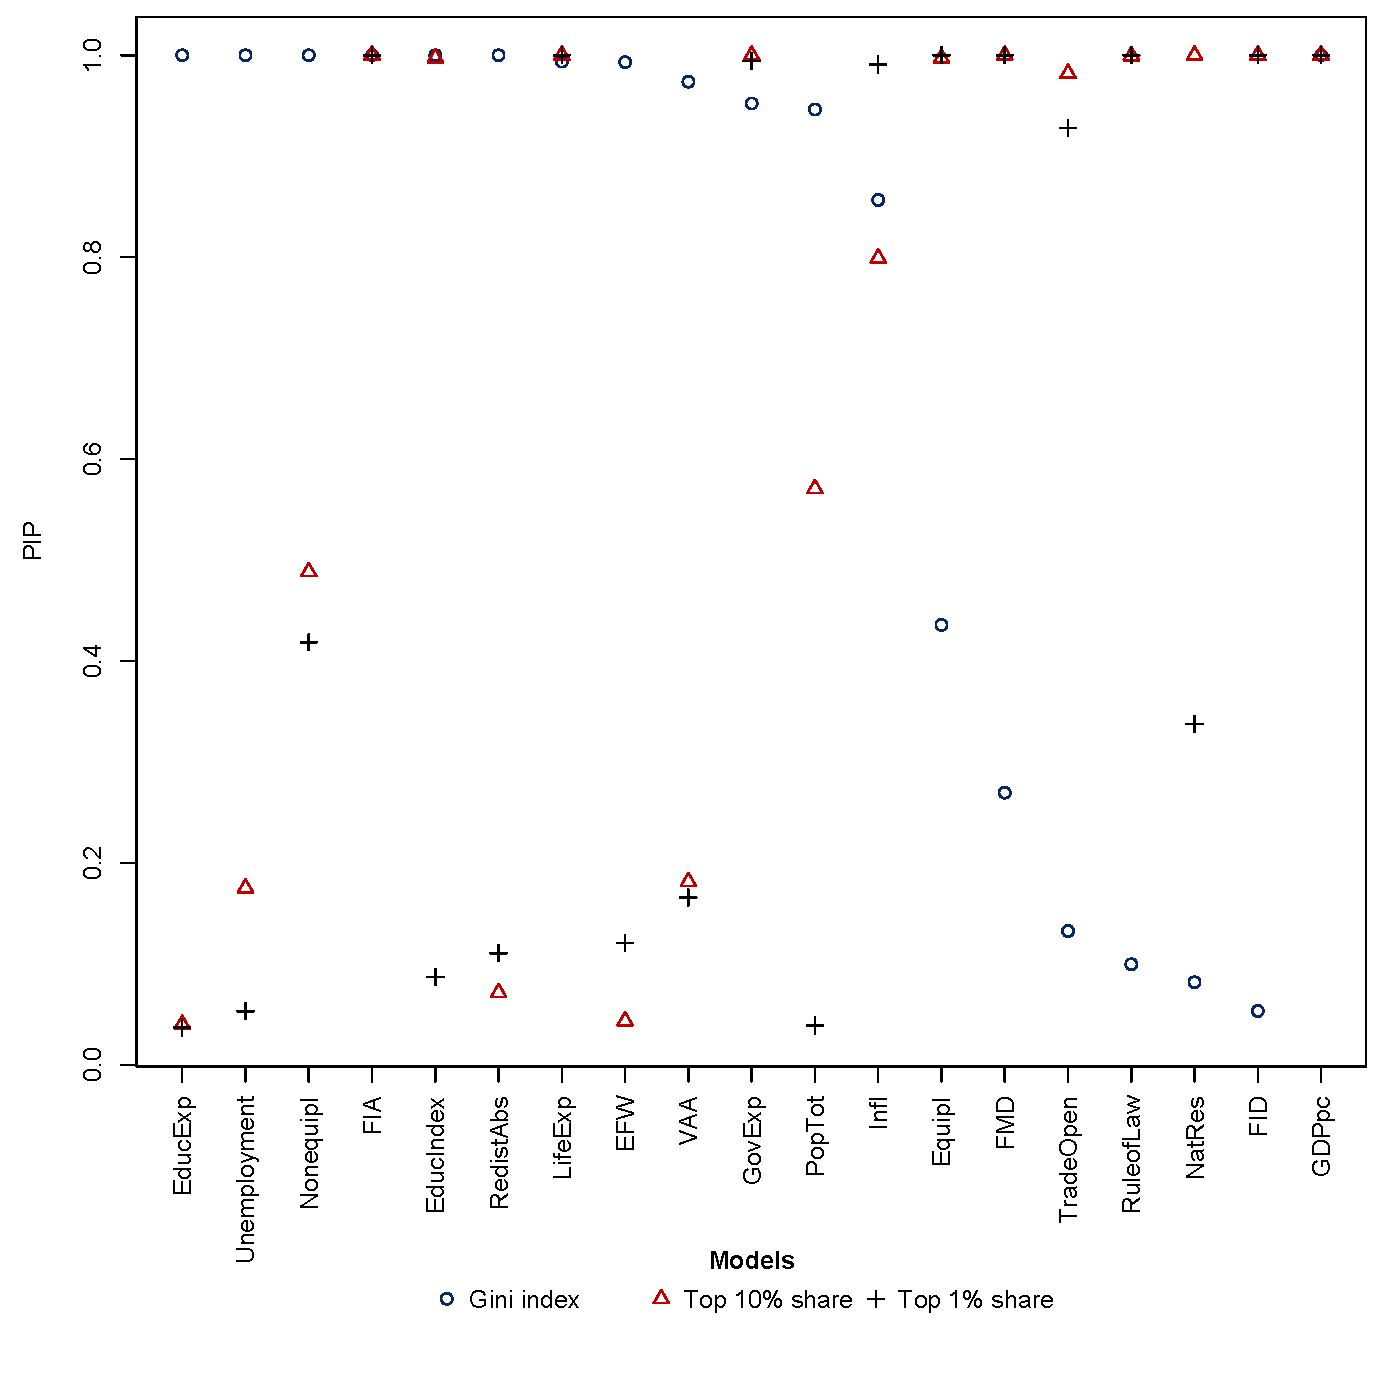
\includegraphics[width=0.8\textwidth, keepaspectratio]{figures/comp_baseline_pip_sel}
  \caption{\acp{PIP} with different inequality measures}
  \label{ch4fig:comp_ineq_sel}
  \begin{minipage}{0.8\textwidth}
    \footnotesize
    \emph{Note: The comparison only shows variables which show \ac{PIP} $> 0.9$ in at least one of the models.}
    \end{minipage}
\end{figure}

\begin{figure}[ht!]
  \centering
  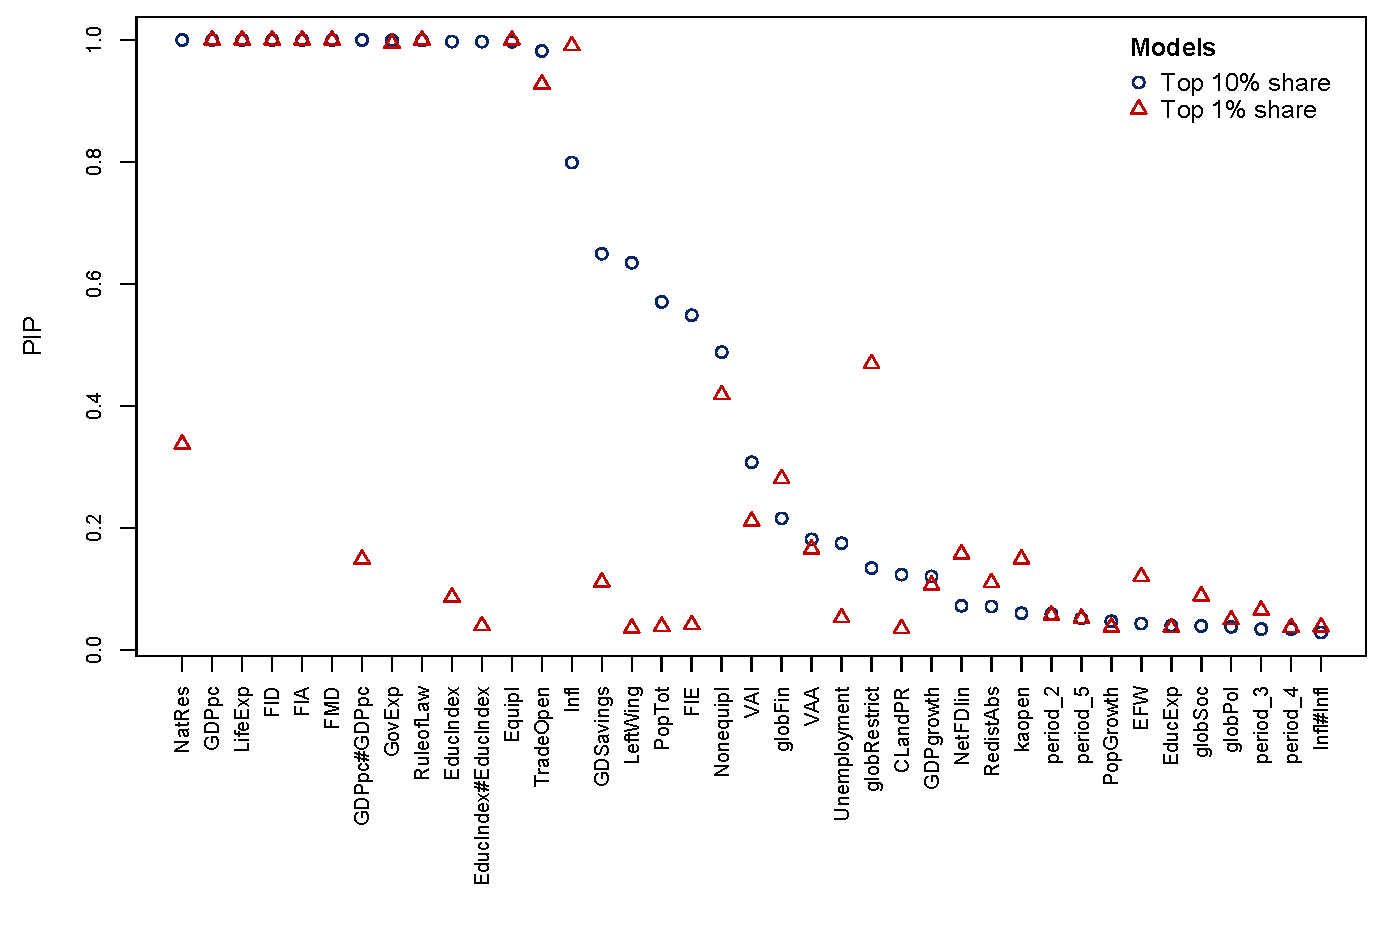
\includegraphics[width=\textwidth, keepaspectratio]{figures/topsh_comparison_all}
  \caption{\acp{PIP} for different top income shares with baseline priors}
  \label{ch4fig:comp_topshares}
\end{figure}

\begin{table}[ht!]
  \caption{BMA, baseline results. Dependent variable Top 1\% share, 394 observations.}\label{ch4res:baseline_top1}
    \footnotesize
    \centering
  \begin{tabular}{lrrr}
    \toprule
                                 & PIP & Post Mean & Post SD \\
    \midrule
  Rule of law & 1.00 & -0.17039 & 0.04688 \\
  GDP per capita & 1.00 & 0.48163 & 0.29090 \\
  Life expectancy & 1.00 & -0.45605 & 0.06980 \\
  Equipment investment & 1.00 & -0.19727 & 0.05526 \\
  Financial institutions depth & 1.00 & 0.16380 & 0.05689 \\ 
  Access to financial institutions & 1.00 & -0.25945 & 0.06419 \\
  Financial markets depth & 1.00 & 0.15454 & 0.04989 \\ 
  Government expenditures & 0.99 & 0.11633 & 0.04718 \\ 
  Inflation & 0.99 & 0.11773 & 0.04922 \\
  Trade openness & 0.93 & 0.10374 & 0.05711 \\ 
  \midrule
  Restrictions on globalization & 0.47 & 0.03804 & 0.05418 \\ 
  Non-equipment investment & 0.42 & 0.03197 & 0.05001 \\ 
  Natural resources rents & 0.34 & -0.02182 & 0.04037 \\ 
  Financial globalization & 0.28 & -0.02001 & 0.04269 \\
  Value added in industry & 0.21 & -0.01389 & 0.03634 \\
  Value added in agriculture & 0.17 & -0.00969 & 0.03053 \\ 
  Net FDI (\% GDP) & 0.16 & -0.00730 & 0.02401 \\
  Chinn-Ito index & 0.15 & 0.00828 & 0.02797 \\
  GDP per capita sq. & 0.15 & -0.08401 & 0.28484 \\
  Economic freedom & 0.12 & -0.00945 & 0.03762 \\ 
  Gross domestic savings & 0.11 & 0.00634 & 0.02688 \\
  Redistribution & 0.11 & 0.00495 & 0.02085 \\
  GDP growth & 0.11 & -0.00504 & 0.02208 \\
  Social globalization & 0.09 & -0.00626 & 0.03233 \\
  Education index (UN) & 0.09 & -0.01003 & 0.07309 \\ 
  % Period 3 & 0.07 & -0.00214 & 0.01452 \\
  % Period 2 & 0.06 & -0.00146 & 0.01249 \\
  Unemployment & 0.05 & 0.00131 & 0.01287 \\ 
  % Period 5 & 0.05 & 0.00140 & 0.01362 \\
  Political globalization & 0.05 & 0.00137 & 0.01473 \\ 
  Financial institutions efficiency & 0.04 & -0.00070 & 0.01024 \\ 
  Education index sq. & 0.04 & 0.01380 & 0.07857 \\ 
  Total population & 0.04 & -0.00060 & 0.01484 \\ 
  Inflation sq. & 0.04 & 0.00053 & 0.01828 \\ 
  Population growth & 0.04 & 0.00020 & 0.00844 \\
  % Period 4 & 0.04 & 0.00019 & 0.00892 \\ 
  Education expenditures & 0.04 & -0.00002 & 0.00935 \\ 
  Left-wing orientation & 0.04 & -0.00028 & 0.00843 \\ 
  Civil liberties \& political rights & 0.04 & 0.00009 & 0.00846 \\
    \bottomrule
  \end{tabular}
\end{table}

The results using the Top 1\% share for top regressors differs in the drop of \acp{PIP} for natural resource rents, and education attainment. We hypothesize that natural resource rents might redistribute the share of income from the top decile to the rest of the distribution without actually affecting the share of the income going to the very top. The top 1\% income earners might well be among the ones enjoying capital rents from the country resources. While education appears to have equalizing income effect for the lower part of the distribution, it is reasonable that it wears out for the very top income earners in the distribution. Figure \ref{ch4fig:comp_topshares} depicts comparison of inclusion probabilities of all variables considered in the estimation for the Top 10\% share and Top 1\% share.

\subsection{Robustness checks}
We perform robustness checks for all three specifications employing alternative model priors\footnote{We also perform robustness checks using alternative hyperparameter $g$ and Markov-chain samplers, but these do not affect our results.}. We choose random and dilution priors to address prior model size concentrated around the mean number of potential regressors and correlation among them by each of the model priors, respectively.

\begin{figure}[ht!]
  \centering
  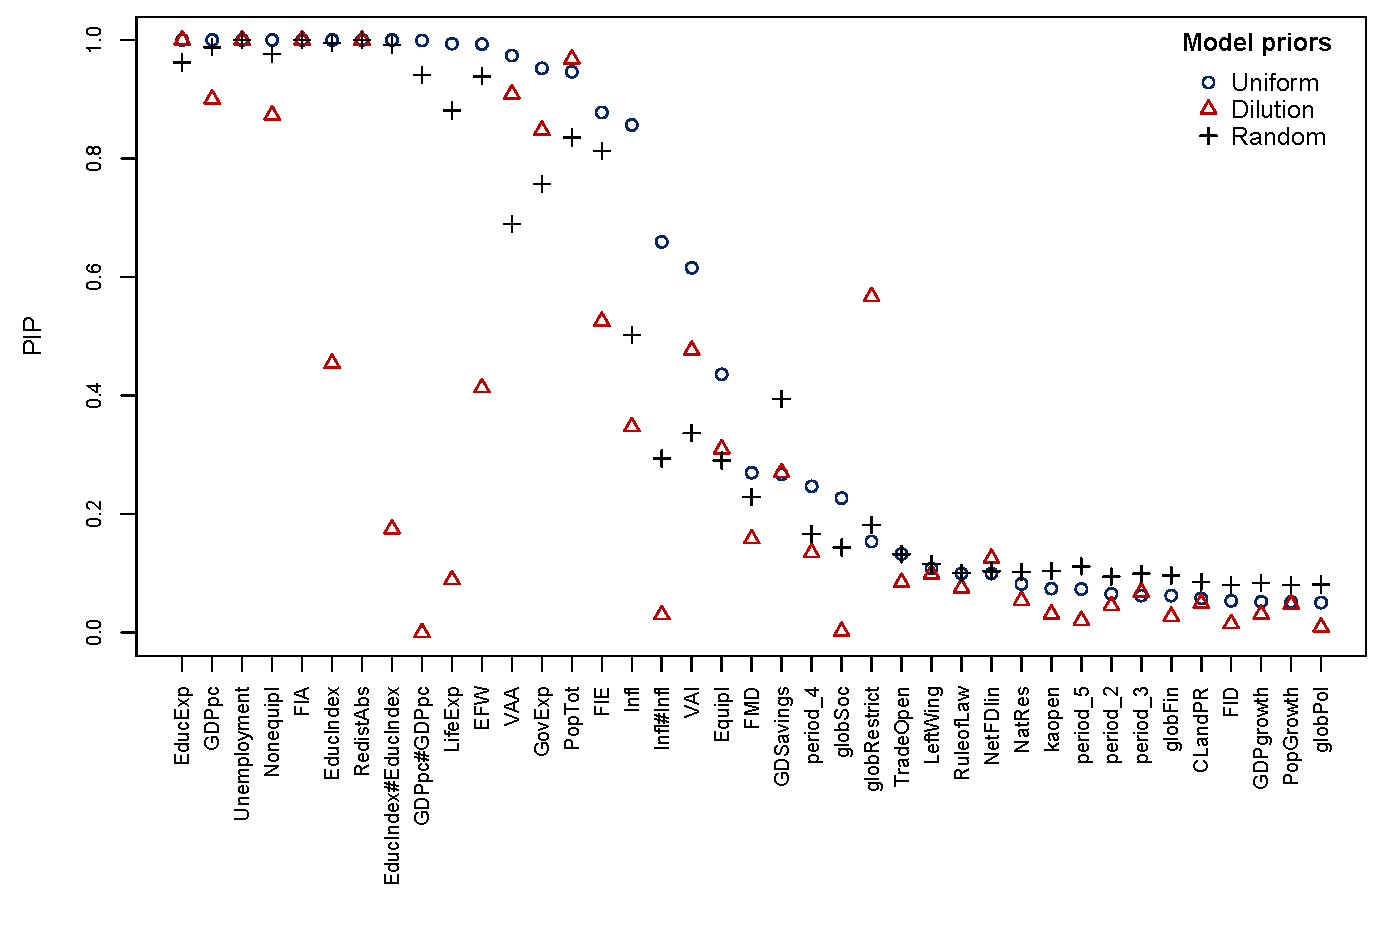
\includegraphics[width=\textwidth, keepaspectratio]{figures/model_priors_comparison_gini}
  \caption{Robustness checks with alternative model priors, Gini coefficient}
  \label{ch4fig:gini_comp}
\end{figure}

\begin{figure}[ht!]
  \centering
  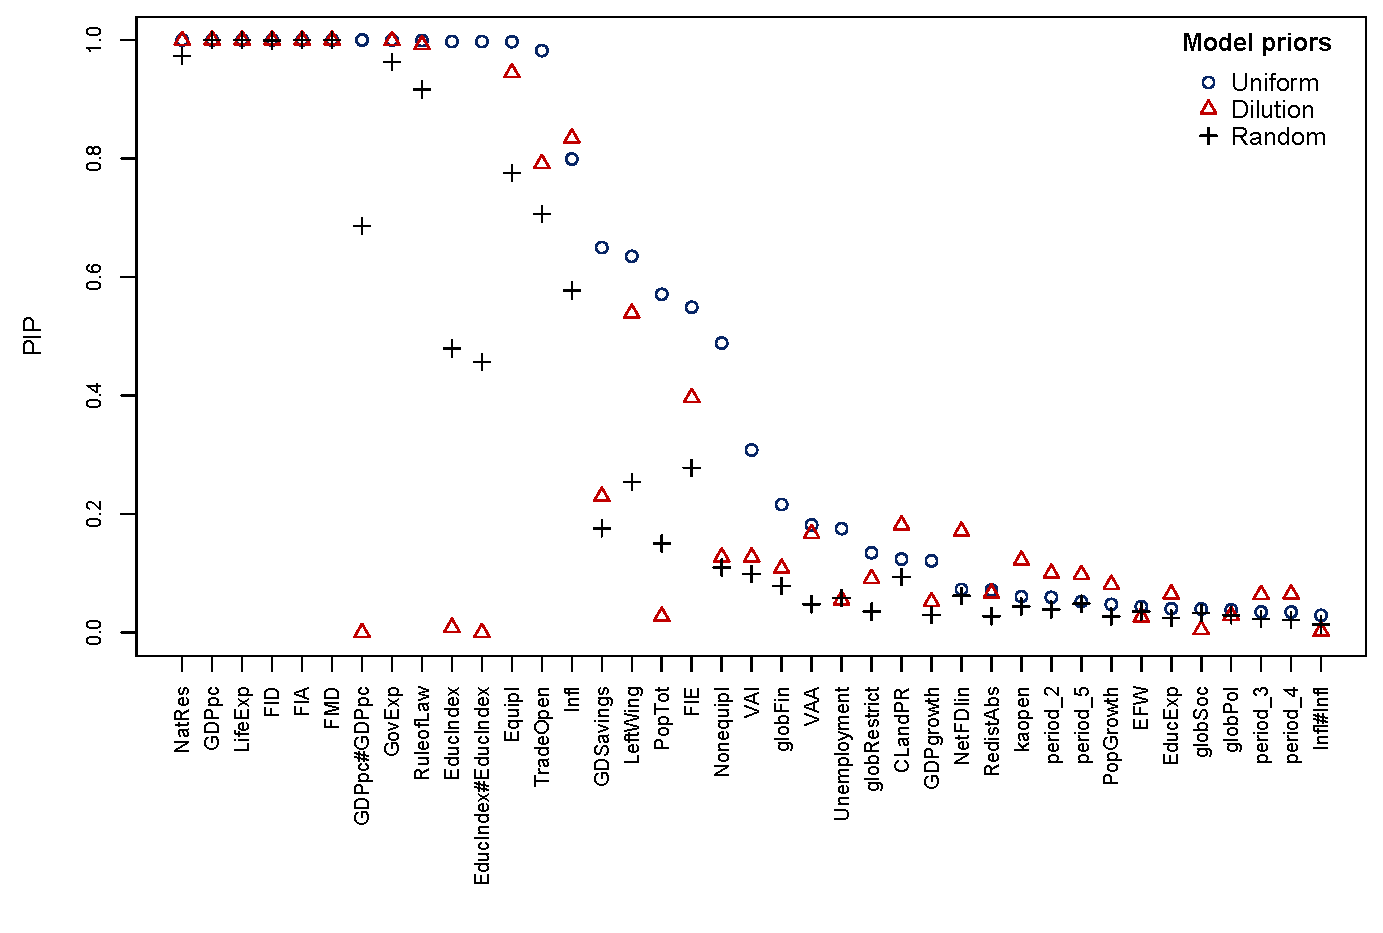
\includegraphics[width=\textwidth, keepaspectratio]{figures/model_priors_comparison_top10}
  \caption{Robustness checks with alternative model priors, Top 10\% share}
  \label{ch4fig:top10_comp}
\end{figure}

\begin{figure}[ht!]
  \centering
  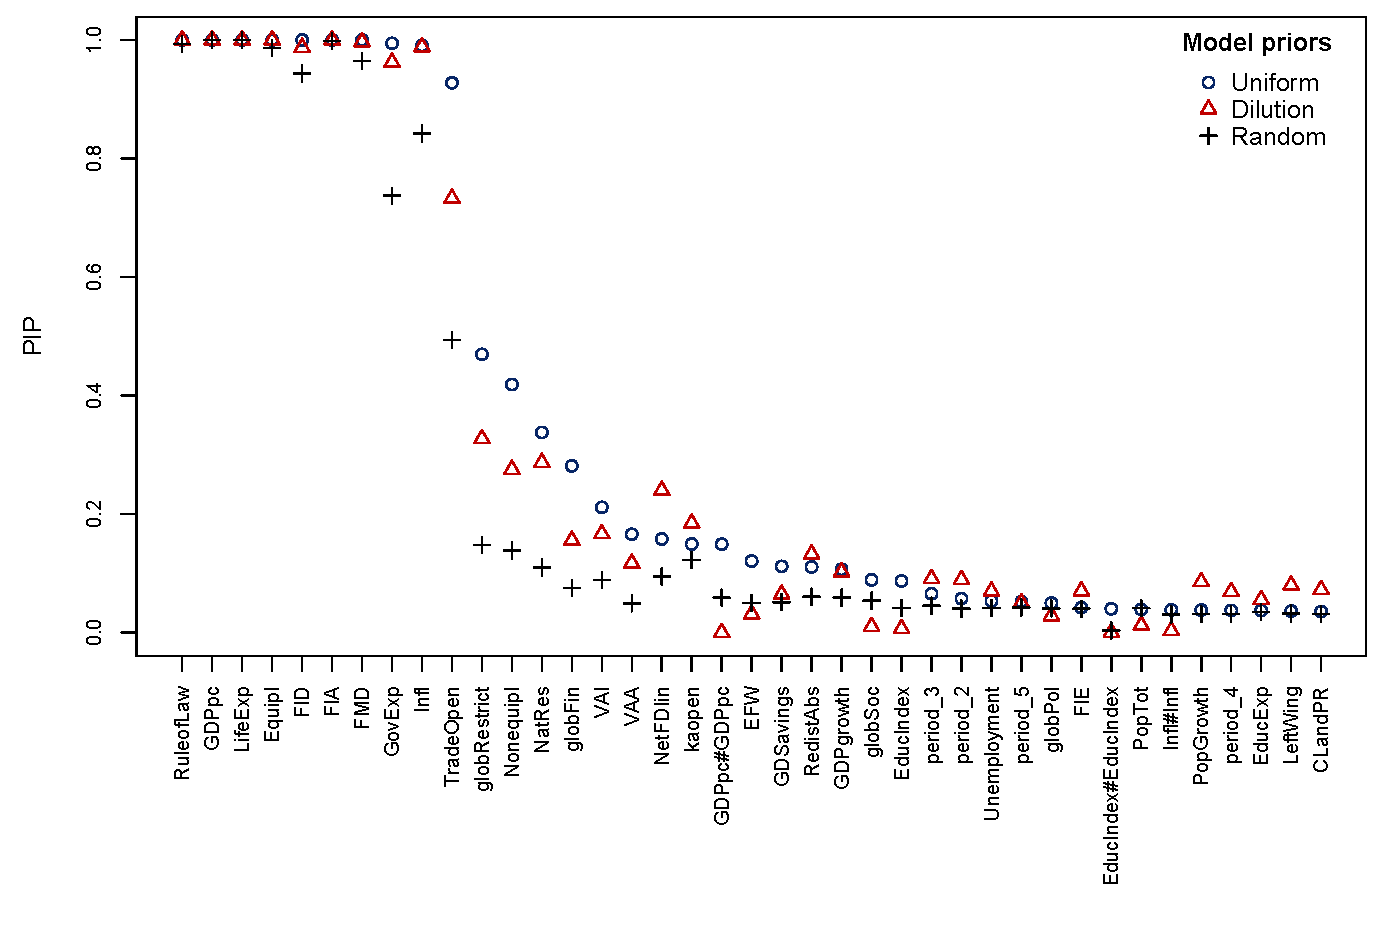
\includegraphics[width=\textwidth, keepaspectratio]{figures/model_priors_comparison_top1}
  \caption{Robustness checks with alternative model priors, Top 1\% share}
  \label{ch4fig:top1_comp}
\end{figure}

The alternative priors influence the results similarly in all three specifications. The random mode prior decreases \acp{PIP} for the regressors as it generally prefers smaller models. Nevertheless, the results are only marginally effected for Gini coefficient as well as the top income shares with a few exception of education index in the case of Top 10\% share and trade openness for both top income shares. The use of dilution model prior which penalizes the models with highly correlated regressors, we see more significant differences. Above all, the quadratic terms show very low inclusion probabilities. That is not surprising since they are correlated with their original values. This irrelevance of quadratic terms is universal across inequality measures and we may argue that it is due to the construction of the concerned variables. While the \acp{PIP} for other regressors remain similar to the baseline in the case of top income shares, for the Gini index of overall income inequality, we observe some regressors which are now penalized by the dilution prior. Taking the set of the important regressors in the baseline specification, we observe drop in the inclusion probability for education index, life expectancy, and economic freedom. Given high correlations among the set of regressors, this is not surprising and allows to narrow down the number of regressors robustly associated with income inequality.

%
%
%
%
%

\section{Conclusion}
\label{ch4sec:conclusion}
In the paper, we explore the robust determinants of income inequality with a special attention given to indicators of financial development. We choose financial indicators that reflect the access, efficiency, and size of financial markets and institutions. We believe that the detailed indicators provide better proxies for the functions of finance - screen investment opportunities, monitor the debtors who were provided funding, as well as pooling and management of risk. We allow for model uncertainty by employing \ac{BMA} and examine a number of other potential determinants of income inequality. 

We show that financial development has complex relationship on income distribution. While access to finance has a universally inequality decreasing effect, the larger size of financial markets and financial institutions associates with higher top income shares, irrelevant for the Gini coefficient of the income distribution. This finding suggests that the size of financial markets also equalizes the income among the first 9 deciles. 

We find a few other important covariates for income inequality. Education, redistribution, and changing demographic structure seem to be linked with lower income inequality. On the contrary, unemployment, investment other than machinery, economic freedom - ease of pursuing economic opportunities, and inflation all positively relate to income inequality. As in the case of financial indicators, we find that the link could be more complex. When looking at the top income shares, some of the covariates (education, unemployment, redistribution, and economic freedom) cease to be relevant, while some other (trade openness, rule of law, and machinery investment) seem to matter.

The results we present warrant caution in drawing quick conclusions on the matter of income inequality determinants. While finance, technology, and trade likely affect the distributional outcomes, it can have varying influence on different parts of the income distribution.

% Finance captures the capacity of financial intermediaries and markets to screen investment opportunities, monitor the debtors who were provided funding, as well as pooling and management of risk. With inequality, the focus of the paper is on the inequality in the distribution of income. Arguably, the literature discusses other concepts of inequality, e.g. intergenerational persistence of relative income differences or equality of opportunity \parencite{demirgucc2009finance}.

% \textcite{kroszneretal2007} show that financial crises have relative more severe impact on the sectors which depend more on external financing. The consequences of crises on firms relate to institutional environment and materialize through lower production capacity and competition.

% Overall, these results suggest that policies seeking to improve the governance and robustness of local banks should be prioritized over size-enhancing reforms from a normative point of view \parencite{gimet2011closer}.

% The benefits of capital markets liberalization seem to be concentrated to the top of the income distribution. Top quintile of the distribution accrues nearly all of the income growth following the liberalization while the share of middle three quantiles decreases and the bottom remains unaffected \parencite{das2003income}.

\clearpage
%
%
%
%
%
%
%
%
%
%
\newpage
\printbibliography
\clearpage
%
%
%
%
%
\appendix
\renewcommand{\thesection}{A\arabic{section}}%
\renewcommand{\thetable}{A\arabic{table}}%
\renewcommand{\thefigure}{A\arabic{figure}}%
\renewcommand{\theequation}{A\arabic{equation}}%
\setcounter{equation}{0}%
\setcounter{table}{0}%
\setcounter{figure}{0}%

\section{Appendix}
\label{ch4sec:appch2}



\subsection*{The composition of financial indicators}
\label{ch4subsec:finind_comp}
\begin{table}[ht!]
    \small
    \caption{Underlying Components of Financial Development Indicators}
    \label{ch4tab:finind}
    \centering
    \begin{tabular}{ll}
      \toprule
      \textsc{Indicator} & \textsc{Measure} \\
      \midrule
      \multicolumn{2}{l}{\textbf{Financial institutions}} \\
      \midrule
      \multirow{2}{*}{Access} 	& Bank branches per 100,000 adults \\
                                  & ATMs per 100,000 adults \\
      \midrule
      \multirow{6}{*}{Efficiency}		& Net interest margin \\
                                  & Lending-deposits spread \\ 
                                  & Noninterest income to total income \\
                                  & Overhead costs to total assets \\
                                  & Return on assets \\
                                  & Return on equity \\
            
      \midrule
      \multirow{4}{*}{Depth}	& Domestic private credit to the real sector to the GDP \\
                                  & Pension fund assets/GDP \\
                                  & Mutual fund assets/GDP \\
                                  & Insurance premiums life and nonlife/GDP \\
      \midrule
      \multicolumn{2}{l}{\textbf{Financial markets}} \\
      \midrule
      \multirow{6}{*}{Depth} 	& Stock market capitalization/GDP \\
                                  & Stocks traded/GDP \\
                                  & International debt securities of government/GDP \\
                                  & Total debt securities of financial corporations/GDP \\
                                  & Total debt securities of nonfinancial corporations/GDP \\
      \bottomrule
    \end{tabular}
\end{table}

\clearpage
\subsection*{Dataset description}
\begin{center}
\footnotesize
\begin{longtable}{l p{0.50\linewidth} p{0.3\linewidth}}
    \caption{List of variables}
    \label{ch4app:exog} \\
    \toprule 
  Variable & Definition (+ optional comments) & Source \\
    \midrule 
  GiniNet & After\-tax Gini index based on distribution of income (The Standardized World Income Inequality Database). & \href{http://fsolt.org/swiid/}{Solt (2019)} \\
  GiniMarket & Before-tax Gini index based on distribution of income  (The Standardized World Income Inequality Database). & \href{http://fsolt.org/swiid/}{Solt (2019)} \\	
  Top10share & Share of income going top decile of the distribution. & \href{https://wid.world/}{WID} \\	
  Top1share & Share of income going top percentile of the distribution. & \href{https://wid.world/}{WID} \\
  FIA & Access to financial institutions & \href{http://data.imf.org/?sk=F8032E80-B36C-43B1-AC26-493C5B1CD33B}{\textcite{svirydzenka2016introducing}} \\
  FID & Financial institutions depth & \href{http://data.imf.org/?sk=F8032E80-B36C-43B1-AC26-493C5B1CD33B}{\textcite{svirydzenka2016introducing}} \\
  FIE & Financial institutions efficiency & \href{http://data.imf.org/?sk=F8032E80-B36C-43B1-AC26-493C5B1CD33B}{\textcite{svirydzenka2016introducing}} \\
  FMD & Financial markets depth & \href{http://data.imf.org/?sk=F8032E80-B36C-43B1-AC26-493C5B1CD33B}{\textcite{svirydzenka2016introducing}} \\
  FME & Financial markets efficiency & \href{http://data.imf.org/?sk=F8032E80-B36C-43B1-AC26-493C5B1CD33B}{\textcite{svirydzenka2016introducing}} \\
  GDPpc & Level of GDP per capita & \href{http://data.worldbank.org/indicator/NY.GDP.PCAP.PP.KD}{WB} \\
  NatRes & Total natural resource rents are the sum of oil rents, natural gas rents, coal rents (hard and soft), mineral rents, and forest rents. & \href{http://data.worldbank.org/indicator/NY.GDP.TOTL.RT.ZS}{WB} \\
  PopGrowth & Annual population growth 1980-2009 & \href{http://data.worldbank.org/indicator/SP.POP.GROW}{WB} \\
  GovExp & General government final consumption expenditure (formerly general government consumption). & \href{http://data.worldbank.org/indicator/NE.CON.GOVT.ZS}{WB}\\
  NNSavings & Net national savings (gross national savings less the value of consumption of fixed capital, \% GNI). & \href{http://data.worldbank.org/indicator/NY.ADJ.NNAT.GN.ZS}{WB} \\
  EducExp & Education expenditure refers to the current operating expenditures in education, including wages and salaries and excluding capital investments in buildings and equipment.. & \href{http://data.worldbank.org/indicator/NY.ADJ.AEDU.GN.ZS}{WB} \\
  Infl & Inflation as measured by the consumer price index. & \href{http://data.worldbank.org/indicator/FP.CPI.TOTL.ZG}{WB} \\
  VAA & Agriculture, forestry, and fishing value added (\% GDP). & \href{http://data.worldbank.org/indicator/NV.AGR.TOTL.ZS}{WB} \\
  VAI & Industry value added (\% GDP). & \href{http://data.worldbank.org/indicator/NV.IND.TOTL.ZS}{WB} \\
  GFCF & Gross fixed capital formation (\% of GDP). & \href{http://data.worldbank.org/indicator/NE.GDI.FTOT.ZS}{WB} \\
  NetFDI &  Foreign direct investment, net inflows (\% of GDP). & \href{http://data.worldbank.org/indicator/BX.KLT.DINV.WD.GD.ZS}{WB} \\
  GDPgrowth & Annual growth of GDP. & \href{http://data.worldbank.org/indicator/NY.GDP.MKTP.KD.ZG}{WB} \\
  LifeExp & Life expectancy at birth.  & \href{http://data.worldbank.org/indicator/SP.DYN.LE00.IN}{WB}\\
  LabForce & Total labor force comprises people ages 15 and older who meet the International Labor Organization definition of the economically active population: all people who supply labor for the production of goods and services during a specified period. Labor force total. & \href{http://data.worldbank.org/indicator/SL.TLF.CACT.ZS}{WB} \\
%   PopDens & Population density (people per sq. km of land area). & \href{http://data.worldbank.org/indicator/EN.POP.DNST}{WB} \\
  RuleOfLaw & Rule of law estimate & \href{http://data.worldbank.org/indicator/RL.EST}{WB} \\
  CLandPR & Average of index for civil liberties and political rights & \href{https://freedomhouse.org/report/freedom-world-2016/methodology}{Freedom House} \\
%   OutwardO & Trade (\% of GDP)  & \href{http://data.worldbank.org/indicator/NE.TRD.GNFS.ZS}{WB} \\
  ChinnIto & Chinn-Ito index of financial openness. & \href{http://web.pdx.edu/~ito/Chinn-Ito_website.htm}{Chinn-Ito} \\ 
  LeftWing & Dummy equal to 1 when left oriented party lead the country. & \href{http://www.nsd.uib.no/macrodataguide/set.html?id=11&sub=1}{DPI} \\
  ActivRestrict & Activity restrictions. Regulatory restrictions on bank activities and the mixing of banking and commerce. & \href{http://faculty.haas.berkeley.edu/ross_levine/regulation.htm}{Barth et al. (2013)} \\
  CapitalReg & Capital Regulatory index. & \href{http://faculty.haas.berkeley.edu/ross_levine/regulation.htm}{Barth et al. (2013)} \\
  DiversIndex & Whether there are explicit, verifiable, quantifiable guidelines for asset diversification and banks are allowed to make loans abroad. & \href{http://faculty.haas.berkeley.edu/ross_levine/regulation.htm}{Barth et al. (2013)} \\
  EducIndex & Calculated using mean years of schooling and expected years of schooling & \href{http://hdr.undp.org/en/content/education-index}{UN} \\
  NetInterestMargin & Accounting value of banks' net interest revenue as a share of average interest-bearing assets; a measure of the efficiency of the banking sector. & \href{http://data.worldbank.org/data-catalog/global-financial-development}{GFDD} \\
  BankZScore & return on banks' assets plus the ratio of banks' equity and assets, divided by the standard deviation of the return on assets (ROA+equity/assets)/sd(ROA); a measure of stability of the banking sector & \href{http://data.worldbank.org/data-catalog/global-financial-development}{GFDD} \\
  Privatecredit & Domestic private credit to the real sector to GDP; a measure of the depth of the banking sector & \href{http://data.worldbank.org/data-catalog/global-financial-development}{GFDD} \\
  MarketCap & Value of listed shares to GDP; a measure of the depth of stock markets.& \href{http://data.worldbank.org/data-catalog/global-financial-development}{GFDD} \\
  MarketTurn & Stock market value traded to total market capitalization; a measure of the efficiency of stock markets. & \href{http://data.worldbank.org/data-catalog/global-financial-development}{GFDD} \\
  BankBranches & Number of bank branches per 100,000 adults & \href{http://data.worldbank.org/data-catalog/global-financial-development}{GFDD} \\
  Loan2Deposits & Loan-to-deposit ratio. & \href{http://data.worldbank.org/data-catalog/global-financial-development}{GFDD} \\
  Redist & Difference between market (pre-tax) and net (after-tax0 Gini index based on distribution of income  (The Standardized World Income Inequality Database). & \href{http://fsolt.org/swiid/}{Solt (2016)} \\	
  FinLib & Averaged components of Economic Freedom of the World index 3D (freedom to own foreign currency accounts), 4C (black-market exchange rates), 4D (controls of the movement of capital and people), and 5A (credit market regulations). & \href{https://www.fraserinstitute.org/economic-freedom/dataset}{\textcite{gwartney2017}} \\
  \bottomrule
\end{longtable}
\end{center}

\end{document}